% ====================================================================
%  Introduction (~3 min)
%  Layout convention: text/maths left, figure right.
% ====================================================================

\begin{frame}{Precision medicine: individual predictions}
\begin{columns}[c]
  \begin{column}{0.5\textwidth}
    \small
    \begin{itemize}
      \item Use each patient's own data -- clinical, lifestyle, biomarkers -- instead of one-size-fits-all estimates.
      \item A model trained on past patients gives an \emph{individual} prediction for a new patient.
      \item The clinician uses it alongside other information.
    \end{itemize}
    \vspace{0.5em}
    \textbf{This thesis:} predict \emph{when} an event happens for an individual -- learn
    \[
      \hat S(t \mid \bm{x}) \quad \text{from} \quad \D = \{(\bm{x}_i, t_i, \delta_i)\}_{i=1}^{N}
    \]
  \end{column}
  \begin{column}{0.46\textwidth}
    \centering
    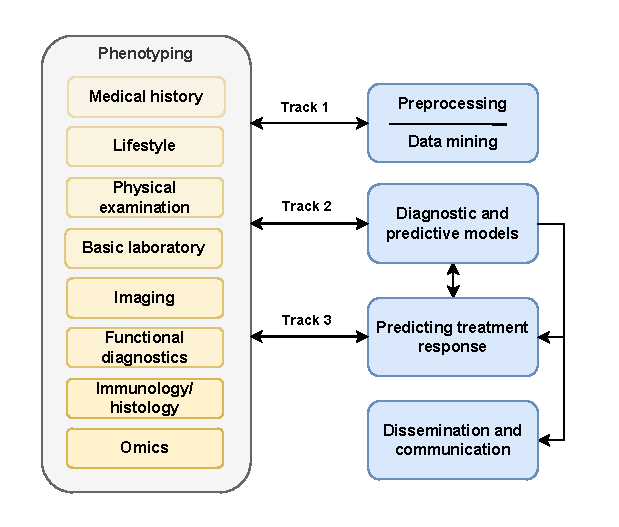
\includegraphics[width=\linewidth,height=0.72\textheight,keepaspectratio]{precision_medicine.pdf}
    \figsource{Figure adapted from K\"onig et al.~\cite{konig_precision_2017}}
  \end{column}
\end{columns}
\end{frame}

\begin{frame}{Predicting \emph{when}, from partly observed data}
\begin{columns}[c]
  \begin{column}{0.58\textwidth}
    \small
    For each individual $i$ we observe
    \[
      t_i = \min(e_i, c_i), \qquad \delta_i = \mathbbm{1}[e_i \le c_i]
    \]
    \vspace{-0.6em}
    \begin{itemize}
      \item $e_i$: event time (death, relapse, a fall, \dots)
      \item $c_i$: censoring time (dropout, end of study)
    \end{itemize}
    \vspace{0.3em}
    \textbf{Right-censored} ($\delta_i = 0$): we only know $e_i > c_i$.
    \vspace{0.3em}

    Dropping censored cases wastes information and biases the estimates -- survival analysis uses them.
  \end{column}
  \begin{column}{0.4\textwidth}
    \centering
    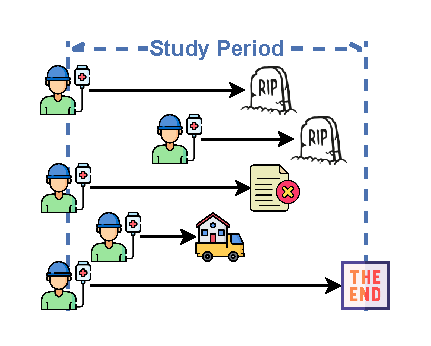
\includegraphics[width=\linewidth]{censoring.pdf}
    \figsource{Figure courtesy of Qi et al.~\cite{qi_current_2025}}
  \end{column}
\end{columns}
\end{frame}

\begin{frame}{Four challenges, four research questions}
\footnotesize
\begin{description}[RQ4.]
  \item[RQ1.] How can machine learning models, and deep survival models in particular, quantify uncertainty in individual predictions?
  \item[RQ2.] How can a single survival model predict the time to multiple events that may be competing or co-occurring, and use temporal ordering information when available?
  \item[RQ3.] How should survival predictions be evaluated when outcomes are censored, and how can evaluation bias be reduced under dependent censoring?
  \item[RQ4.] How can survival prediction methods be applied to censored time-to-event outcomes beyond mortality, specifically time to fall in home care clients and time to degradation in ball bearings?
\end{description}
\vspace{-0.6em}
\roadmap[0.78]{0}
\end{frame}
